% !TEX encoding = UTF-8 Unicode
\level{2}{Fase SD: Software Design}
	\textbf{Periodo}: dal \insdate{05}{03}{2015} al \insdate{03}{04}{2015} \\Questa fase comincia con la fine della \insphase{Fase DI} e termina con l'incontro con il proponente per mostrare l'architettura scelta.\\
	Le attività di questa fase sono:
	\begin{itemize}
		\item \textbf{Norme di Progetto}: Viene fatto un incremento alle norme per poter stendere il documento \insdoc{Specifica Tecnica}. Viene successivamente fatta una verifica/validazione per fissare una baseline al documento che diventerà \insdoc{Norme di Progetto v3.00}.
		\item \textbf{Specifica Tecnica}: Questa attività caratterizza la \insphase{Progettazione Architetturale}. Il \insrole{Progettista} stende la \insdoc{Specifica Tecnica} che contiene le scelte progettuali, ad alto livello, che il progetto dovrà avere. Saranno quindi descritti quali design pattern \projectname{} implementerà, l'architettura generale del software, i principali flussi di controllo e il tracciamento dei requisiti.
		\item \textbf{Glossario}: Viene fatto un incremento al Glossario aggiungendo tutti i vocaboli che si ritiene importante siano inclusi. Viene successivamente fatta una verifica/validazione per fissare una baseline al documento che diventerà \insdoc{Glossario v3.00}.
		\item \textbf{Piano di Qualifica}: L'incremento consiste nell'aggiungere al documento \insdoc{Piano di Qualifica v1.00} il dettaglio dell'esito della \insrev{Revisione dei Requisiti} e la parte della pianificazione dei test. Questa attività genererà, dopo una verifica e validazione, il file \insdoc{Piano di Qualifica v3.00}.
		\item \textbf{Piano di Progetto}: l'incremento che sarà fatto al documento \insdoc{Piano di Progetto} in questa fase consiste nell'apportare correzioni nella divisione delle attività e stillare il consuntivo di questo periodo. Dopo un'accurata verifica che fisserà una nuova baseline e la validazione il documento diventerà \insdoc{Piano di Progetto v3.00}.
	\end{itemize}
	\level{3}{Diagramma di Gantt delle attività}
	\begin{figure}[H]\centering
		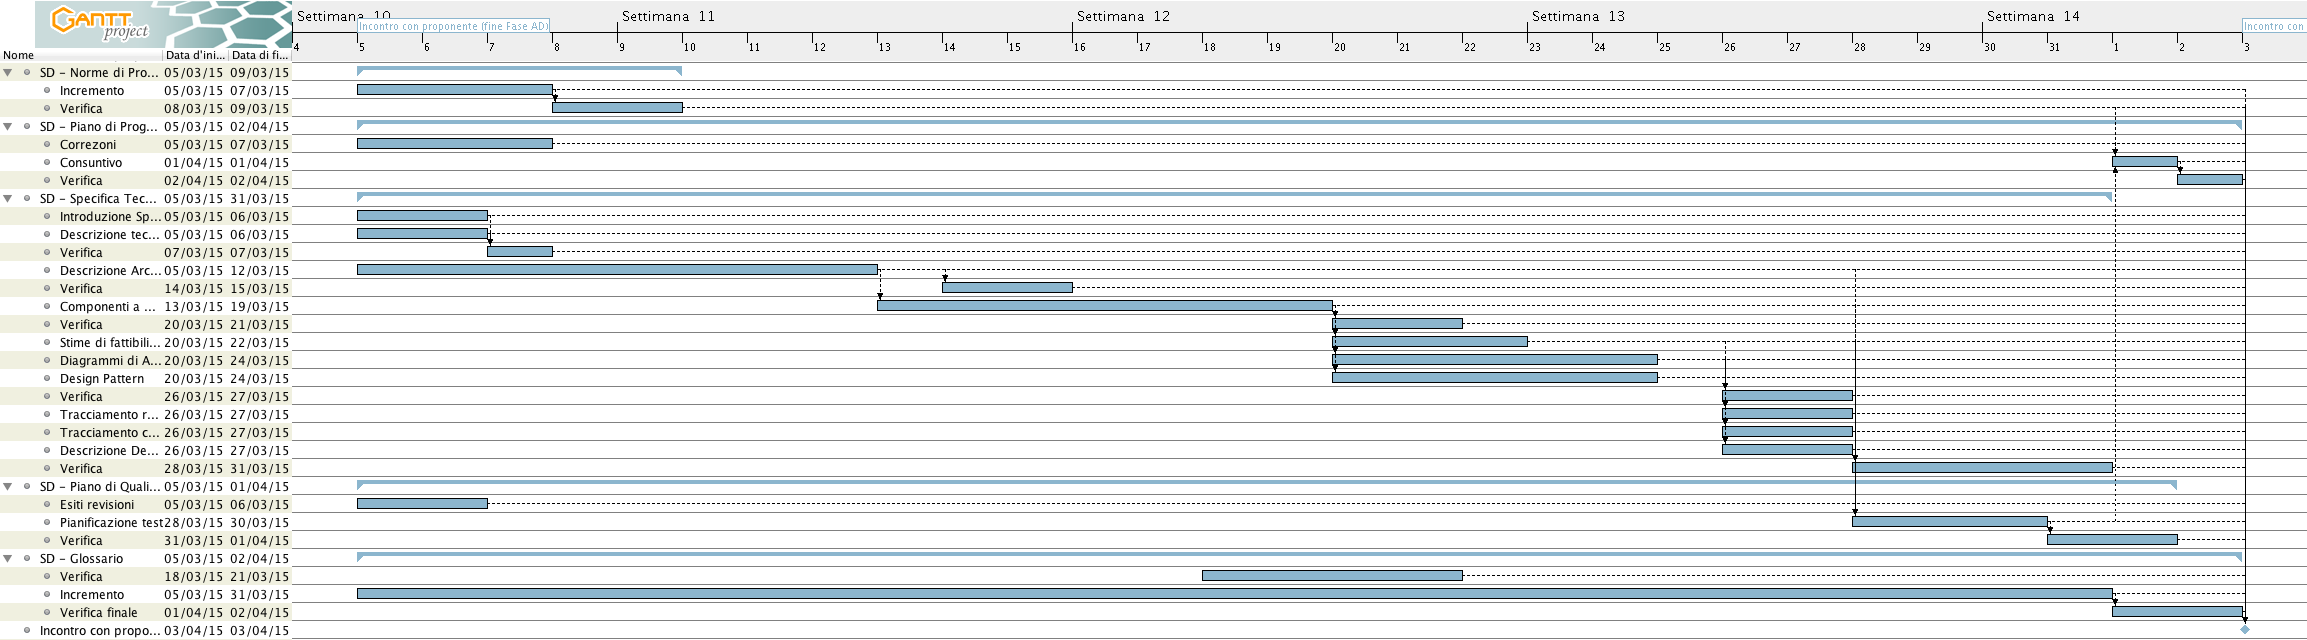
\includegraphics[width=\textwidth]{PianoDiProgetto/Pics/FaseSD.png}
	\caption{Gantt Fase SD}
\end{figure}
